\documentclass{beamer}

\usepackage[french]{babel}
\usepackage[utf8]{inputenc}
\usepackage[T1]{fontenc}
\usepackage{amsmath, amsthm, amsfonts}
\usepackage{siunitx}
\usepackage{tikz}
\usepackage{hyperref}
%\usepackage[backend=biber, autocite=footnote]{biblatex}
\usepackage{xcolor}
\usepackage{caption}
\usepackage{booktabs}
\usepackage{mathtools}

\tikzset{>=latex}
\usetikzlibrary{calc,decorations.pathreplacing}
\sisetup{locale=FR, per-mode=symbol}

\newcommand{\abs}[1]{\left| #1 \right|}
%\renewcommand{\vec}[1]{\ensuremath{\overrightarrow{\boldsymbol{\mathrm{ #1 }}}}}
\newcommand{\rhat}{\vec{\hat{r}}}
\newcommand{\xhat}{\vec{i}}
\newcommand{\yhat}{\vec{j}}
\newcommand{\zhat}{\vec{k}}
\newcommand{\real}{\mathbb{R}}
\newcommand{\der}[2]{\frac{\mathrm{d}#1}{\mathrm{d}#2}}
\newcommand{\pder}[2]{\frac{\partial #1}{\partial #2}}
\newcommand{\dif}{\mathrm{d}}
\newcommand{\ddif}{\,\mathrm{d}}
\newcommand{\grad}{\vec{\nabla}}
\newcommand{\exemple}[1]{\begin{fullwidth}#1\end{fullwidth}}
\newcommand{\norm}[1]{\lVert #1 \rVert}
\newcommand{\vu}{\vec{u}}
\newcommand{\vv}{\vec{v}}
\newcommand{\vr}{\vec{r}}
\newcommand{\va}{\vec{a}}
\newcommand{\vF}{\vec{F}}
\newcommand{\vecxyz}[3]{#1 \xhat + #2 \yhat + #3 \zhat}
\newcommand{\vecxy}[2]{#1 \xhat + #2 \yhat}

\theoremstyle{definition}
\newtheorem*{defn}{Definition}



\begin{document}

\begin{frame}
  \frametitle{La première loi de Newton}
  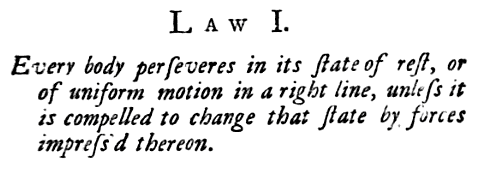
\includegraphics[scale=0.6]{newton1stlaw.png}
\end{frame}


\begin{frame}
  \frametitle{Force nette}

  On considère une boîte de pizza qu'essaient de s'arracher trois personnes tel
  qu'indiqué dans la figure ci-dessous.  Le module de la force exercée par Han
  est de \SI{9}{\newton}, celui de la force exercée par Leia est de
  \SI{4}{\newton}, et celui de la force exercée par Luke est \SI{8}{\newton}.

  Déterminer la force nette qui agit sur la boîte de pizza.

  \begin{center}
  \begin{tikzpicture}
    \begin{scope}[scale=0.8]
      \draw (-1, -1) rectangle (1, 1);
      \begin{scope}[shift={(0, -0.6)}]
        \draw[red] (0, 0) -- ++(60:1) arc (60:120:1) -- cycle;
        \filldraw[brown, rounded corners=0.7] (59:0.9) -- (59:1)
          arc (59:121:1) -- (121:0.9) arc (121:59:0.9);
        \clip (0, 0) -- ++(60:0.9) arc (60:120:0.9) -- cycle;
        \fill[red!60!black] (65:0.4) circle (0.1);
        \fill[red!60!black] (100:0.73) circle (0.1);
        \fill[red!60!black] (78:0.85) circle (0.1);
        \fill[red!60!black] (110:0.5) circle (0.1);
        \fill[red!60!black] (110:0.2) circle (0.1);
      \end{scope}
      \node at (0, 0.6) {PIZZA};
      \draw[very thick, ->] (-1, 0.3) -- (-3, 1.5) node[left] {$\vec{F}_\mathrm{Luke}$};
      \draw (-1, 0.7) arc (90:150:0.4);
      \node at (-1.32, 0.85) {\SI{60}{\degree}};
      \draw[very thick, ->] (-1, -1) -- (-2, -2) node[left] {$\vec{F}_\mathrm{Leia}$};
      \draw[dashed] (-1, -1) -- (-1, -2);
      \draw (-1, -1.5) arc (-90:-135:0.5);
      \node at (-1.3, -1.8) {\SI{45}{\degree}};
      \draw[very thick, ->] (1, 0.1) -- ++(20:2.8) node[right] {$\vec{F}_\mathrm{Han}$};
      \draw[dashed] (1, 0.1) -- (3, 0.1);
      \draw (1.8, 0.1) arc (0:20:0.8);
      \node at (2.2, 0.3) {\SI{20}{\degree}};
    \end{scope}
    \begin{scope}[scale=0.8, shift={(6, -3)}]
      \uncover<2->{
        \draw[->] (0, -1) -- (0, 2.4) node[left] {$y$};
        \draw[->] (-2, 0) -- (3.1, 0) node[below] {$x$};
        \begin{scope}[shift={(1, -0.3)}]
          \draw[very thick, ->] (-1, 0.3) -- (-3, 1.5) node[left] {$\vec{F}_\mathrm{Luke}$};
          \draw (-1, 0.7) arc (90:150:0.4);
          \node at (-1.32, 0.85) {\SI{60}{\degree}};
        \end{scope}
        \begin{scope}[shift={(1, 1)}]
          \draw[very thick, ->] (-1, -1) -- (-2, -2) node[left] {$\vec{F}_\mathrm{Leia}$};
          \draw (-1, -1.5) arc (-90:-135:0.5);
          \node at (-1.3, -1.8) {\SI{45}{\degree}};
        \end{scope}
        \begin{scope}[shift={(-1, -0.1)}]
          \draw[very thick, ->] (1, 0.1) -- ++(20:2.8) node[right] {$\vec{F}_\mathrm{Han}$};
          \draw (1.8, 0.1) arc (0:20:0.8);
          \node at (2.2, 0.3) {\SI{20}{\degree}};
        \end{scope}}
      \uncover<3->{
        \draw[red, ->] (200:1.8) -- (20:4) node[below] {$x'$};
        \draw[red, ->] (-70:1) -- (110:3) node[left] {$y'$};
        \draw[red] (110:1.3) arc (110:150:1.3);
        \node[red] at (130:1.6) {\SI{40}{\degree}};
        \draw[red] (200:0.8) arc (200:225:0.8);
        \node[red] at (212.5:1.2) {\SI{25}{\degree}};
      }
    \end{scope}
  \end{tikzpicture}
  \end{center}

\end{frame}


\begin{frame}
  \frametitle{La deuxième loi de Newton}
  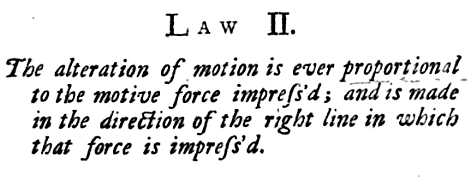
\includegraphics[scale=0.6]{newton2ndlaw.png}
\end{frame}

\begin{frame}
  \frametitle{Ascenseur}

  Un câble d'acier tire un ascenseur pour qu'il monte à vitesse constante, tel
  qu'illustré dans la figure suivante.

  \begin{columns}
    \begin{column}{0.20\textwidth}
        \begin{tikzpicture}[>=latex, scale=0.25]
          \draw[fill=black] (0, 3) circle (7pt);
          \draw (0, 3) circle (10pt);
          \draw[ultra thick] (-0.23, 2.9) -- (-0.23, 0);
          \draw[ultra thick] (-1.23, -3) rectangle (0.77, 0);
          \draw (-3.23, 1) -- (-1.4, 1) -- (-1.4, -3.5);
          \draw (2.77, 1) -- (0.94, 1) -- (0.94, -3.5);
          \draw (-2.23, 1) -- (-2, 2.4) -- (-0.32, 3);
          \draw (1.77, 1) -- (1.54, 2.4) -- (0.35, 3);
          \draw[very thick, ->] (1.4, -2.5) -- node[right] {$\vv$} (1.4, -0.5);
          \draw[->] (4, 2) node[right] {câble} -- (-0.2, 1);
        \end{tikzpicture}
    \end{column}
    \begin{column}{0.70\textwidth}

      Tous les effets de frottements sont négligeables.
      Quel énoncé est vrai?
    \end{column}
  \end{columns}

  \begin{enumerate}
    \item la force du câble dirigée vers le haut est plus grande que la force de
      gravité dirigée vers le bas.
    \item la force du câble dirigée vers le haut est égale à la force de gravité
      dirigée vers le bas.
    \item la force du câble dirigée vers le haut est plus petite que la force de
      gravité dirigée vers le bas.
    \item la force du câble dirigée vers le haut est plus grande que la somme de
      la force de gravité dirigée vers le bas et de la force dirigée vers le bas
      causée par l'air.
    \item aucune de ces réponses. L’ascenseur monte car le câble raccourcit et
      non à cause d'une force vers le haut exercée par le câble sur l'ascenseur.
  \end{enumerate}
\end{frame}


\begin{frame}
  \frametitle{Pizza Rapido}

  On considère une boîte de pizza qu'essaient de s'arracher trois personnes tel
  qu'indiqué dans la figure ci-dessous.  Le module de la force exercée par Han
  est de \SI{9}{\newton}, celui de la force exercée par Leia est de
  \SI{4}{\newton}, et celui de la force exercée par Luke est \SI{8}{\newton}.

  La masse de la boîte de pizza est de \SI{2.00}{kg}.  Déterminer
  l'accélération de la boîte de pizza.

  \begin{center}
  \begin{tikzpicture}
    \begin{scope}[scale=0.8]
      \draw (-1, -1) rectangle (1, 1);
      \begin{scope}[shift={(0, -0.6)}]
        \draw[red] (0, 0) -- ++(60:1) arc (60:120:1) -- cycle;
        \filldraw[brown, rounded corners=0.7] (59:0.9) -- (59:1)
          arc (59:121:1) -- (121:0.9) arc (121:59:0.9);
        \clip (0, 0) -- ++(60:0.9) arc (60:120:0.9) -- cycle;
        \fill[red!60!black] (65:0.4) circle (0.1);
        \fill[red!60!black] (100:0.73) circle (0.1);
        \fill[red!60!black] (78:0.85) circle (0.1);
        \fill[red!60!black] (110:0.5) circle (0.1);
        \fill[red!60!black] (110:0.2) circle (0.1);
      \end{scope}
      \node at (0, 0.6) {PIZZA};
      \draw[very thick, ->] (-1, 0.3) -- (-3, 1.5) node[left] {$\vec{F}_\mathrm{Luke}$};
      \draw (-1, 0.7) arc (90:150:0.4);
      \node at (-1.32, 0.85) {\SI{60}{\degree}};
      \draw[very thick, ->] (-1, -1) -- (-2, -2) node[left] {$\vec{F}_\mathrm{Leia}$};
      \draw[dashed] (-1, -1) -- (-1, -2);
      \draw (-1, -1.5) arc (-90:-135:0.5);
      \node at (-1.3, -1.8) {\SI{45}{\degree}};
      \draw[very thick, ->] (1, 0.1) -- ++(20:2.8) node[right] {$\vec{F}_\mathrm{Han}$};
      \draw[dashed] (1, 0.1) -- (3, 0.1);
      \draw (1.8, 0.1) arc (0:20:0.8);
      \node at (2.2, 0.3) {\SI{20}{\degree}};
    \end{scope}
    \begin{scope}[scale=0.8, shift={(6, -3)}]
      \begin{scope}[shift={(1, -0.3)}]
        \draw[very thick, ->] (-1, 0.3) -- (-3, 1.5) node[left] {$\vec{F}_\mathrm{Luke}$};
      \end{scope}
      \begin{scope}[shift={(1, 1)}]
        \draw[very thick, ->] (-1, -1) -- (-2, -2) node[left] {$\vec{F}_\mathrm{Leia}$};
      \end{scope}
      \begin{scope}[shift={(-1, -0.1)}]
        \draw[very thick, ->] (1, 0.1) -- ++(20:2.8) node[above] {$\vec{F}_\mathrm{Han}$};
      \end{scope}
      \draw[->] (200:1.8) -- (20:4) node[below] {$x$};
      \draw[->] (-70:1) -- (110:3) node[left] {$y$};
      \draw (110:1.3) arc (110:150:1.3);
      \node at (130:1.6) {\SI{40}{\degree}};
      \draw (200:0.8) arc (200:225:0.8);
      \node at (212.5:1.2) {\SI{25}{\degree}};
    \end{scope}
  \end{tikzpicture}
  \end{center}

\end{frame}


\begin{frame}
  \frametitle{La troisième loi de Newton}
  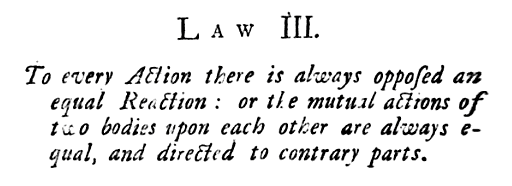
\includegraphics[scale=0.6]{newton3rdlaw.png}
\end{frame}


\begin{frame}
  \frametitle{Tire la Terre}

  La force gravitationnelle terrestre sur un objet de masse $m$ à la surface
  de la Terre est donnée par
  \[
    F_g = mg
  \]
  en direction du centre de la Terre ($g = \SI{9.8}{\meter/s^2}$).

  Si vous sautez dans les airs, la Terre exerce une force sur vous qui vous
  fait accélérer.  Vous exercez également une force sur la Terre qui la fait
  accélérer.

  Calculez
  \begin{columns}
    \begin{column}{0.65\textwidth}
      \begin{itemize}
        \item la force que la Terre exerce sur vous
        \item la force que vous exercez sur la Terre
        \item l'accélération que vous subissez
        \item l'accélération que la Terre subit
      \end{itemize}
    \end{column}
    \begin{column}{0.5\textwidth}
      \uncover<2>{
      \begin{itemize}
        \item[] \alert{\SI{598}{\newton} vers la Terre}
        \item[] \alert{\SI{598}{\newton} de la Terre vers moi}
        \item[] \alert{\SI{9.80}{m/s^2} vers la Terre}
        \item[] \alert{\SI{1.00e-22}{m/s^2} de la Terre vers moi}
      \end{itemize}
    }
    \end{column}
  \end{columns}
\end{frame}

\end{document}

